%%%%%%%%%%%%%%%%%%%%%%%%%%%%%%%%%%%%%%%%%
% Thin Formal Letter
% LaTeX Template
% Version 2.0 (7/2/17)
%
% This template has been downloaded from:
% http://www.LaTeXTemplates.com
%
% Author:
% Vel (vel@LaTeXTemplates.com)
%
% Originally based on an example on WikiBooks 
% (http://en.wikibooks.org/wiki/LaTeX/Letters) but rewritten as of v2.0
%
% License:
% CC BY-NC-SA 3.0 (http://creativecommons.org/licenses/by-nc-sa/3.0/)
%
%%%%%%%%%%%%%%%%%%%%%%%%%%%%%%%%%%%%%%%%%

%----------------------------------------------------------------------------------------
%	DOCUMENT CONFIGURATIONS
%----------------------------------------------------------------------------------------

\documentclass[11pt]{letter} % 10pt font size default, 11pt and 12pt are also possible

\usepackage{graphicx}

\usepackage[hidelinks, colorlinks=false]{hyperref}

\usepackage{geometry} % Required for adjusting page dimensions

\longindentation=0pt % Un-commenting this line will push the closing "Sincerely," to the left of the page

\geometry{
	paper=letterpaper, % Change to letterpaper for US letter
	top=1.2cm, % Top margin
	bottom=2cm, % Bottom margin
	left=2cm, % Left margin
	right=2cm, % Right margin
	%showframe, % Uncomment to show how the type block is set on the page
}

\usepackage[T1]{fontenc} % Output font encoding for international characters
\usepackage[utf8]{inputenc} % Required for inputting international characters

\usepackage{palatino} % Use the Stix font by default

\usepackage{microtype} % Improve justification

\usepackage{setspace}

\setstretch{1.22}

%----------------------------------------------------------------------------------------
%	YOUR NAME & ADDRESS SECTION
%----------------------------------------------------------------------------------------

\signature{\\ Ralf J. Sommer, PhD \\ Director, MPI for Biology T\"{u}bingen \\ Adjunct Professor, \\ University of T\"{u}bingen} % Your name for the signature at the bottom

% \address{Ricardo Azevedo \\ Dept. Biology \& Biochemistry \\ University of Houston
% \\ Houston, TX 77204-5001, USA} % Your address and phone number

\address{
\includegraphics[trim= 3.5in 0.5in 0in 0in, scale=0.4]{./cover_letter_figs/MPI_logo.png} \\ Director: Ralf J. Sommer \\ \footnotesize Max-Planck-Ring 9, D-72076 T\"{u}bingen, Germany \\ \footnotesize Tel: ++49 7071 601371; Fax: ++49 7071 601498 \\ \footnotesize E-mail: ralf.sommer@tuebingen.mpg.de}

%----------------------------------------------------------------------------------------


\renewcommand{\closing}[1]{\par\nobreak\vspace{\parskip}%
  \stopbreaks
  \noindent
  \ifx\@empty\fromaddress\else
  \hspace*{\longindentation}\fi
  \parbox{\indentedwidth}{\raggedright
  		 \ifx\@empty\fromsigimg
  		   \ignorespaces #1\\[6\medskipamount]%
  		 \else
  		   \ignorespaces #1\\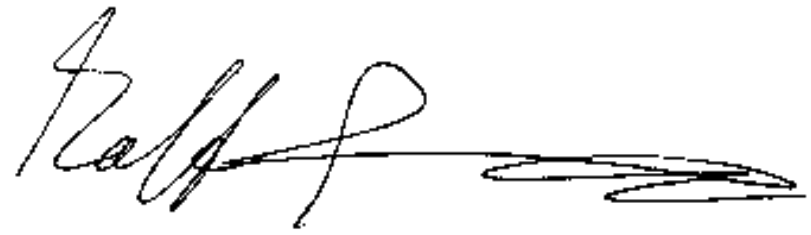
\includegraphics[height=8\medskipamount]{./cover_letter_figs/ralf_signiture.png}
  		 \fi
       \ifx\@empty\fromsig
           \fromname
       \else \fromsig \fi\strut}%
   \par}


\begin{document}

%----------------------------------------------------------------------------------------
%	ADDRESSEE SECTION
%----------------------------------------------------------------------------------------


\begin{letter}{Dr. Feilim Mac Gabhann \& Prof. Jason Papin \\ Editors-in-Chief \\ \emph{PLOS Computational Biology}}

%----------------------------------------------------------------------------------------
%	LETTER CONTENT SECTION
%----------------------------------------------------------------------------------------


\opening{Dear Editors,}

We would like to submit to \emph{PLOS Computational Biology}, our manuscript entitled ``Spatial and temporal heterogeneity alters the cost of plasticity in \emph{Pristionchus pacificus}''.

The prevalence of developmental (phenotypic) plasticity in nature has been thoroughly documented\footnote{West-Eberhard, 2003}. However, many unanswered questions remain with respect to ecological and evolutionary consequences of phenotypic plasticity. A major contention in this regards has been the concept of the cost of plasticity, i.e., the intrinsic fitness cost of a developmentally-plastic system in contrast to a non-plastic alternative \footnote{DeWit et al., Trends Ecol. Evol., 1998; Forsman, Heredity, 2015; Murren et al., Heredity, 2015}. In a previous contribution, we utilized an integrative approach, combining experimental and theoretical tools, to demonstrate a clear case of the cost of plasticity in the hermaphroditic nematode \emph{Pristionchus pacificus}\footnote{Dardiry et al., Evol. Lett., Volume 7, Issue 1, 2023, Pages 48–57}.

\emph{P. pacificus} forms teeth-like denticles that result in two alternative mouth morph phenotypes, i.e. cannibalistic or non-predatory morphs. Over the last decade, my lab has shown that this dimorphism is experimentally tractable\footnote{Bento et al., Nature, 2010} and we identified the gene regulatory network of plasticity through a series of forward and reverse genetic screens\footnote{Ragsdale et al., Cell, 2013; Sieriebriennikov et al., Cell Rep., 2018}. In addition, the cannibalistic behavior has proven to be genotype-specific with an associated self-recognition system\footnote{Lightfoot et al., Science 2019}.

In this manuscript, we present a stage-structured metapopulation model based on the experimentally-derived data from \emph{P. pacificus}. To fully understand the ecological consequences of the cost of plasticity in \emph{P. pacificus}, we introduce both spatial and temporal heterogeneity with respect to the resource type. We highlight how such heterogeneity can alleviate the cost of phenotype and result in transient coexistence and even competitive exclusion of the non-plastic genotype. Our work adds a novel case study to the growing literature on the role of phenotypic plasticity in shaping ecological communities and its importance in fluctuating environment.  

% It should be noted that a previous version of this work was submitted in November of last year to \emph{Proceedings of the Royal Society B} (RSPB-2022-1826, handled by Dr. Locke Rowe). Although the manuscript was rejected after review, the comments of the two anonymous reviewers provided invaluable feedback. This prompted us to substantially revise our approach, resulting in the current manuscript that incorporates many of the suggestions of the reviewers, especially the reviewer number 2. In our view, with this major revision, the current manuscript will be a valuable contribution to the body of work on the role of plasticity in ecology and evolution. In addition, a major concern raised with respect to the previous manuscript was the fact that it was an extension of a work that had not been peer reviewed; however, in the mean time, that work has been published in \emph{Evolution Letters}$^3$.

We submit a format-neutral version of our manuscript that contains all the relevant documents. There is no competing interest for any of the authors. The the codes used for data analysis and simulations are available at \url{https://github.com/Kalirad/MetaPopProjection}. 

This work was funded by the Max-Planck Society.

As potential reviewers we would recommend any of the following:

% \footnotesize

\begin{description}
    \item[Ehab Abouheif$^{\ast\dag}$] 
    McGill University 
    (ehab.abouheif@mcgill.ca) 

    \item[Charlotte T. Lee$^{\dag\ddag}$] 
    Duke University 
    (charlotte.t.lee@duke.edu) 

    \item[Hannah Schneider$^{\ast\dag}$] 
    Wageningen University
    (hannah.schneider@wur.nl)

    \item[Roberto Salguero-Gómez$^{\ast\dag\ddag}$] 
     University of Oxford
    (rob.salguero@zoo.ox.ac.uk)
    
    % \item[Brett Melbourne$^{\dag\ddag}$] 
    % University of Colorado Boulder
    % (brett.melbourne@colorado.edu)

    % \item[Jonathan Levine$^{\ast\dag\ddag}$] 
    % Princeton University 
    % (levinej@princeton.edu)

    \item[Andrea Scharf$^{\ddag}\clubsuit$] 
    Missouri University of S \& T 
    (scharfa@mst.edu)

    % \item[Thorsten Wiegand$^{\dag\ddag}$] 
    % Helmholtz Centre for Environmental Research 
    % (thorsten.wiegand@ufz.de)

    % \item[Tom E.X. Miller$^{\dag\ddag}$] 
    % Rice University
    % (tom.miller@rice.edu)

    % \item[Teppo Hiltunen$^{\dag\ddag}$] 
    % University of Turku
    % (teppo.hiltunen@utu.fi)

    \item[Simon Hart$^{\ast\dag\ddag}$] 
    The University of Queensland 
    (s.hart@uq.edu.au)
    


    
\end{description}

Areas of expertise: $^\ast$Phenotypic plasticity.
$^\dag$Ecology.
$\ddag$Computational biology.
$\clubsuit$Nematology.

\normalsize

\vspace{2\parskip}

% None of the materials in this submission have been published or are under consideration for publication elsewhere.  

% We have no conflicts of interest.

% All code and data will be made available at \url{https://github.com/Kalirad/PriPOP}.

We look forward to hearing from you.

\vspace{2\parskip} % Extra whitespace for aesthetics

\closing{Sincerely,}

\vspace{2\parskip} % Extra whitespace for aesthetics

% \ps{P.S. You can find additional information attached to this letter.} % Postscript text, comment this line to remove it

% \encl{Copyright permission form} % Enclosures with the letter, comment this line to remove it

%----------------------------------------------------------------------------------------

\end{letter}
 
\end{document}
